\documentclass[10pt, a4paper]{article}
\usepackage{lrec}
\usepackage{multibib}
\newcites{languageresource}{Language Resources}
\usepackage{graphicx}
\usepackage{tabularx}
\usepackage{soul}
\usepackage{color}
% for eps graphics

\usepackage{verbatim} % comment environment

\usepackage{subcaption} % subfigure

\usepackage[normalem]{ulem} % overstrike \sout{..}

\usepackage{epstopdf}
\usepackage[utf8]{inputenc}

\usepackage{hyperref}
\usepackage{xstring}

\usepackage[dvipsnames]{xcolor}

\newcommand{\secref}[1]{\StrSubstitute{\getrefnumber{#1}}{.}{ }}

\newcommand{\dan}[1]{{\color{Fuchsia}{Dan: #1}}}

\newcommand{\elena}[1]{{\color{BrickRed}{Elena: #1}}}

\newcommand{\mats}[1]{{\color{Blue}{Mats: #1}}}

\newcommand{\normAnn}[0]{our tool }

\title{Towards Transformation-based Annotation of Norm Deviations \\ in an Infrastructure for Research on Swedish as a Second Language}

%\title{Transformation-based Annotation of Norm Deviations \\ in an Infrastructure for Research on Swedish as a Second Language}

\name{Dan Rosén\textsuperscript{1},
      Mats Wirén\textsuperscript{2},
      Elena Volodina\textsuperscript{1}}

\address{\textsuperscript{1}Språkbanken, University of Gothenburg, \textsuperscript{2}Stockholm University \\
         \textsuperscript{1}Box 200, 40530 Göteborg, \textsuperscript{2}SE-10691 Stockholm \\
         dan.rosen@svenska.gu.se, mats.wiren@ling.su.se, elena.volodina@svenska.gu.se\\
         }

\abstract{
This paper describes ongoing work on a tool % the \normAnn system
for annotation of norm deviations (errors) in second-language learner texts, a key component in an intended infrastructure for research on Swedish as a second language. Unlike traditional approaches which treat this as a single task applied to a static learner text, our approach is divided into two steps to reflect the conceptual structure of the problem: a) normalisation  of the learner text by transforming (editing) it to reflect the target hypotheses, and b) the actual norm-deviation annotation, supported by visualisation of the differences between source and normalisation. Another distinct feature of our approach is that a parallel text is generated in the transformation step, with word alignments inferred from the editing operations. This parallel text is a useful resource in its own right, by allowing for search in either or both of the source and normalised texts, and for training of systems for automated annotation of norm deviations. We describe the normalisation component of \normAnn and outline the associated component for annotation of norm deviations currently being implemented. %, as well as the overall intended workflow. %[181 words out of 200 allowed]
\newline
\Keywords{second language learner corpora, error annotation, normalisation}}

\begin{document}

\maketitleabstract

\section{Introduction}

%\mats{Jag kommenterade bort ganska mycket text i sektion 1 och före detta 2 (som var Related work) för att hålla oss inom given plats. Elena, säg till om du vill göra annorlunda. Nuvarande sektion 1 behöver fortfarande ses över; jag lämnar den så här fredag kväll, säg till om du vill att jag ska fixa till den i helgen. }

%\elena{Right now if we take away all "named" comments and merge Conclusions with Discussion, we will already have 4 pages. I will have a fresh look at this later - do not promise I will have a chance during the weekend, though.}

%This work is carried out within the SweLL project, whose goal is to construct an electronic research infrastructure for Swedish as a second language. We take an electronic research infrastructure to consist of the following components:

%\\[10pt]

%-- freely accessible data in electronic format;

%-- a set of tools for data collection and processing, including
%analysis of proficiency levels, norm-deviation (error) annotation, and linguistic annotation;

%-- a technical platform for exploring the data with tools for data analysis and visualization;

%--  expertise within the relevant areas.
%\\
% \begin{enumerate}
% \item freely accessible data in electronic format;
% \item a set of tools for data collection and processing, including analysis of proficiency levels, norm-deviation (error) annotation, and linguistic annotation;
% \item a technical platform for exploring the data with tools for data analysis and visualization;
% \item expertise within the relevant areas.
% \end{enumerate}

The need for data is omnipresent in language-technology projects, not the least when it comes to data produced by second-language learners.
% Not only is the L2 data sensitive in nature and requires (agreements for use of) associated socio-demographic information, but it
Automatic analysis of learner data is very challenging, however, since part-of-speech taggers and syntactic parsers are almost always trained on the standard language. Annotation of norm deviations (that is, errors\footnote{We use the term {\em norm deviation} rather than "error" as a neutral term with respect to the idiosyncrasies of the interlanguage of the learner \cite{Selinker1972}. Similarly, we refer to the changes imposed on a learner text to reflect the norms of the target language as {\em normalisation}. }) is therefore predominantly a manual process. Like all manual annotation, it is very time-consuming, but the problem is exacerbated by the high degree of subjectivity in deciding what the deviation is and of what the correct form would then be.

This paper describes % a tool, \normAnn,
\normAnn which aims at a more efficient handling of normalisation and annotation of norm deviations, thereby alleviating some of the data bootleneck. The work is carried out in the context of a project for constructing an infrastructure for research on Swedish as a second language (SweLL\footnote{%Research Infrastructure for Swedish as a Second Language,
{\tt https://spraakbanken.gu.se/eng/swell\_infra}}), in which \normAnn will constitute a key component.

%In this paper we develop the idea of \textit{transformation-based normalization} of learner texts as a primary step in annotation of norm deviations.
%The origins of the term go to a predecessing pilot within SweLL project \cite{correctAnnotator}, where the idea of logging user actions while editing learner essays was suggested, which in turn has been inspired by the Arabic tool QAWI \cite{QAWI}. We argue that this method is user-friendly and is effective in optimizing manual annotation process through prompting the annotation of norm deviations by comparing original and normalized versions of the same text.

%The rest of the paper is structured as follows: in the next section we set the development of our tool into the context of other available tools for annotation of norm deviations. Motivation behind  transformation-based approach to text normalization is provided in section \ref{sec:targethypothesis} The design of the tool (its prototype) is described in section \ref{sec:norm_tool}, followed by the principles for annotation of norm deviations in section \ref{sec:ann_tool} We conclude the paper with discussion and conclusions.

%\section{Related work}
%\label{sec:relatedwork}

%(Manual) annotation of data for various Language Technology and Digital Humanities projects is a recurring task, which has resulted in a huge number of tools that support annotation of data. Some of the tools are tailored to a particular project need (REFs), others are more generic (REFs). Some drawbacks of generic annotators, e.g. WebAnno (REF) or BRAT (REF) consist in their
%...tricky annotation process; annotations are not structurable and not recyclable; no annotation statistics; no options to perform searches on annotations themselves

%Reusing project-specific tools for other - similar - projects may entail problems with data formats and lacking (bidirectional) interoperability between the tools, undermining effectiveness of their use \elena{, as for example, was the case in MERLIN project with reuse of PAULA, Exmaralda, and FALKO excel plugin\footnote{Information obtained through personal communication with Merlin collaborators and access to their analysis of the used technology, documented in the "Black Book"} (REFS; REFS; REFS)}.

%On the other hand, tools developed for seemingly unrelated areas, for example for annotation parallel corpora (e.g. REF), can provide a number of solutions and insights - especially, if L2 corpora are viewed as two parallel versions: original one, that is, written by the learner, and normalized one, that is, a version of the same text with expert introduced corrections.

% (save for later) A number of existing frameworks for annotation, such as XXX, offer a possibility to build on top of them and adjust to the project aims.

%Related work: various tools in Merlin, exmaralda, Johannes Gräen (multilingual parallel corpus, initial project on Europarl), BRAT (label tokens and draw dependency trees) (http://brat.nlplab.org/index.html) / opensource framework BRAT (Stenetorp et al., 2012)- annotation schemes can be defined for various purposes, including essay marking (Cf. Kutuzov & Kuzmenko, 2015), , webanno (a layer on top of BRAT), annotateit.org, diigo.com,Sacodeyl (http://www.um.es/sacodeyl/en/pages/software.htm);

% (for an overview of error annotation schemes and their implementation, see Lüdeling and Hirschmann, 2015,

Annotation of norm deviations in second-language learner texts is typically done with a purpose-built editing tool, using a hierarchical set of error categories \cite{Granger2008}. For example, in ASK \cite{tenfjord2006ask}, the editor used is the XML editor Oxygen, customised with pop-up menus that reflect the chosen set of error categories. Specifically, annotation of an error involves inserting an XML
{\em sic} tag with a {\em type} attribute encoding the error category, a {\em desc} attribute endoding the error subcategory, and a {\em corr} attribute encoding the correct (normalised) form of the token or tokens. By running a set of XSLT scripts, the XML file can be translated to an HTML format which can be viewed in a web browser, thereby facilitating proofreading of the annotation.

The basic problem with this kind of approach is that it conflates the conceptually separate stages of (traditionally speaking) error coding, namely, error detection, correction and annotation
% Corder 1974
\cite[page 266]{Ellis1994,Granger2008}. This is because correction (normalisation, based on a target hypothesis) is carried out as a subtask of error annotation instead of as an independent task, prior to and separate from error annotation. Also, since normalisations are only a by-product of error annotations, the corrected text as a whole is not readily available for inspection after each annotation step, and as a result it may be more difficult to produce a consistent normalisation.

In Falko \cite{ludeling05multi-levelerror} and MERLIN \cite{MERLIN2014}, target hypothesis corrections have a more independent status in the sense that they are entered in a separate step prior to error annotation, but the normalised text still does not seem to be available in its entirety.

To circumvent these problems, and to reduce subjectivity and increase interannotator agreement, our approach is based on dividing error coding into two steps: normalising the text by transforming (editing) it into a corrected form according to some given criteria, and annotating the norm deviations corresponding to the changes. Furthermore, as a result of this process, a parallel corpus consisting of the learner source text and the normalised text is incrementally constructed. Thus, our contribution is a system for transformation-based annotation of norm deviations which includes the following two components:

\begin{itemize}
\item An editor in which a learner source text can be normalised and a parallel corpus of the two texts is simultaneously generated (Sections~\ref{sec:targethypothesis} and \ref{sec:norm_tool}).
\item Integrated with this, a facility for annotating the normalisations (changes) with norm-deviation categories. (Section~\ref{sec:ann_tool})
\end{itemize}}


\section{Target Hypotheses}
\label{sec:targethypothesis}

%\dan{Highlight that the produced resource is actually a parallel corpus?} \elena{Yes!}

%Text normalisation as a term means transforming original text to some standard form, where standards can be defined differently according to the task at hand, e.g. for tranfsorming written text into speech \cite{sproat2016rnn}. Target hypotheses (TH) in L2 context are interpretations of the learner text (ORIG), e.g.:
%\begin{center}
%\textsc{ORIG: My mother have help us.}

%\textsc{TH1: My mother can help us.}

%\textsc{TH2: My mother has helped us.}
%\end{center}
 %\mats{Jag tror att vi här vill ha ett exempel där TH1 och TH2 är lika troliga, men här uppfattar jag att TH2 är troligare? Ett sådant exempel fanns i fotnot 2 -- jag flyttade hit det i stället.}

As pointed out above, annotation of a norm deviation always involves an interpretation of what the deviation is -- the target hypothesis, here realised by editing of the text. A complication is that there may be multiple competing target hypotheses for a deviation. An example of this from \newcite[Section 2.1]{ludeling05multi-levelerror} is "die Erklärung für diese Phänomen ist einfach", where "diese Ph{\"a}nomen" in absence of other information could equally likely be interpreted as a gender error (with the target hypothesis "dieses Ph{\"a}nomen") or as a number error (with the target hypothesis "diese Ph{\"a}nomene"). Although \normAnn only handles one target hypothesis, in principle we could deal with multiple hypotheses by maintaining different normalisations for a given part of the source text.

Furthermore, some systems allow for several levels of target hypotheses. In the Czech learner corpus of \newcite{Hana2012} a first level normalises grammatical forms without context information. All other deviations (e.g.\ word order) belong to a second level and take the whole sentence into consideration.
In MERLIN \cite{MERLIN2014} two levels are used: a) minimal corrections pertaining only to orthographic and grammatical errors and b) corrections to handle sociolinguistic, lexical and pragmatic deviations to arrive at what is referred to as an acceptable text. Again, \normAnn does not handle this, but it would be possible to do so by maintaining several levels of aligned normalisations. The first level (with basic corrections) would then be aligned to the source text, and the second level (with additional corrections) would be aligned to the first level.

\mats{Dan, I think this paragraph belongs to Section 3 -- do you need anything of it there? Otherwise we should skip it.}
We allow editing operations of characters and tokens, involving insertions, deletions, substitutions % \textcolor{red}{EV:("substitution" instead of "replacement"?; merge? split? - separate actions or as variants of replacement, insertion and deletion?)} and move \textcolor{red}{EV:(Is it a term?)}
or moves (see Section~\ref{sec:norm_tool}), all along creating a parallel version of the original text. By keeping track of the sequence of edit operations, an additional advantage could be gained, namely, that a preliminary error annotation can be automatically inferred (see Section~\ref{sec:ann_tool}). %This is something that we plan to explore later on in the project.
%\dan{Move this overview of the paper to section 1?}

\mats{Dan, I think this paragraph belongs to Section 3 -- do you need anything of it there? Otherwise we should skip it.}
It might be argued that insertions, deletions and
replacements could be computed automatically from the differences between the source and normalised texts, but moves of tokens (which we need in order to keep track of word-order changes) result in added complexity \cite{ShapiraStorer2007} and ambiguities, which is why we log the editing operations.

\begin{figure*}
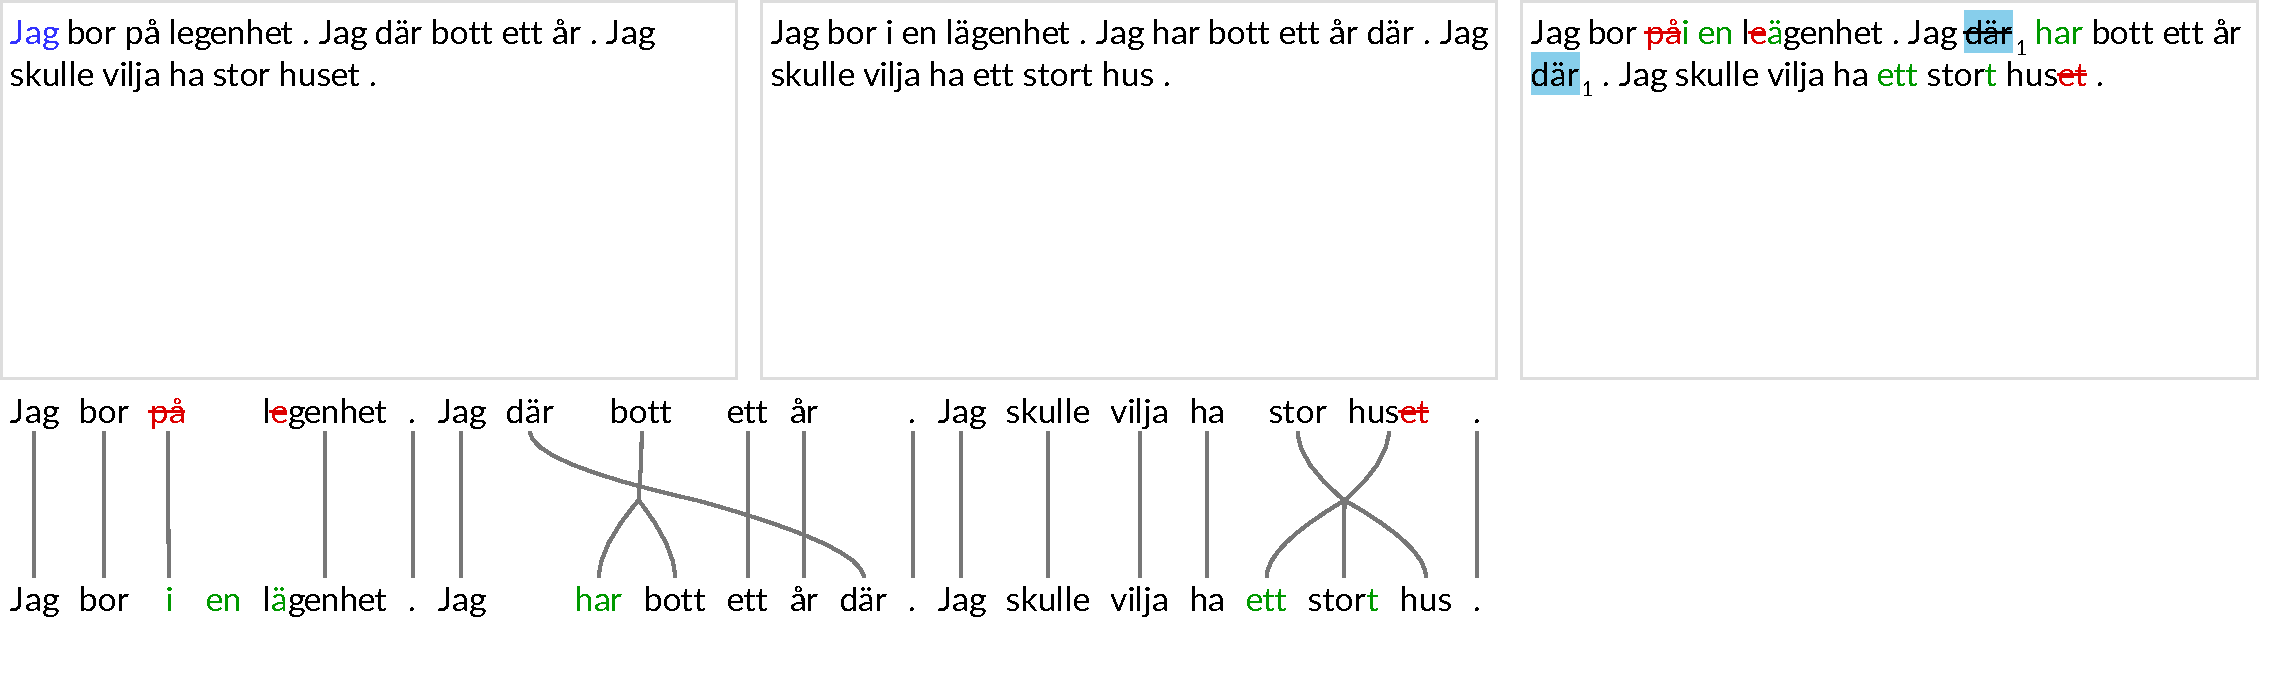
\includegraphics[width=\textwidth, trim={0 0.6cm 0 0}, clip]{screenshot.pdf}
\emph{\small I live in an apartment. I have lived there for one year. I would like to have a big house.}
\caption{Screenshot of an editing session in progress. The three panes in the upper row are from left to right:
1) the source text which cannot be edited,
2) the target hypothesis which is where the annotators do all their edits,
3) a calculated view of the differences between the two texts obtained from the history of edits.
Below the panes we display the the differences pictorially:
the source text on top and the target hypothesis below, with edges
showing how words have been moved.
% Deletions are shown in \textcolor{red}{red} with \sout{overstrike},
% insertions in \textcolor{green}{green} with \underline{underline}.
% (If the text is too long only the current sentence is shown.)
\label{fig:screenshot}
}
\end{figure*}

%We also do not handle multiple {\em competing} target hypotheses for the same source material in the manner of \newcite[Section 2.1]{ludeling05multi-levelerror}.\footnote{An example of this from \newcite[Section 2.1]{ludeling05multi-levelerror} is "die Erklärung für diese Phänomen ist einfach", where "diese Ph{\"a}nomen" in absence of other information could equally likely be interpreted as a gender error (with the target hypothesis "dieses Ph{\"a}nomen") or as a number error (with the target hypothesis "diese Ph{\"a}nomene").} In principle, this could be dealt with in our approach by maintaining different normalisations on the same level for a given part of the source text.

\section{The Normalisation Tool}
\label{sec:norm_tool}
% \dan{Should we name the tool?} \elena{That would be great. Any ideas? SweLL-norm?}
% \mats{NormAnn} \elena{I like NormAnn - refers both to normalization and to annotation}

To normalise a source text using our tool the annotator uses
the text area in the middle of Figure~\ref{fig:screenshot}.

The important thing to understand is that the annotator only need to edit
within this text area, which works just like a text field in a normal program.

Each edit the user does in this text area is reflected in the underlying
parallel structure and shown pictorially in the graph below, which tracks
edits and word order changes between the source and the target text.
The source text is shown on top and the target hypothesis text below, with
edges linking connected words together.

To illustrate what edits we support we this example sentence in English:
``\emph{Examples high light here lotsof futures}''
and see how we can normalise this using our tool by simply editing in
the text area.  Initially the source and target hypotheses text are
the same and each word is connected to itself and the diagram looks as
Figure~\ref{fig:features0}.

\begin{figure}
\centering
\newcommand{\features}[2]{
\begin{subfigure}[t]{0.5\textwidth}
\includegraphics[height=1.8cm, trim={-0.5cm 0.55cm 0 0}, clip]{#1.pdf}
\caption{#2 \label{fig:#1}}
\end{subfigure}
}

\features{features0}{The initial state.}
\features{features1}{Normalising spelling.}
\features{features2}{Normalising oversplitting.}
\features{features3}{Normalising overcompounding.}
\features{features4}{Normalising word order.}
\features{features5}{Inserting missing word.}
\features{features6}{Alternative analysis to illustrate redundant word.}
\caption{Example editing.}
\end{figure}

\begin{itemize}
\item {\it Deviant spelling}: normalise by editing the text.
In Figure~\ref{fig:features1} the user has removed a characted
and inserted two new.

\item {\it Oversplitting}: normalise by removing spaces.
Two words have been merged in Figure~\ref{fig:features2}.

\item {\it Overcompounding}: normalise by inserting spaces.
Two words have been split in Figure~\ref{fig:features3}.

\item {\it Word order}: normalise by drag and drop. Cut and paste can also be used.
The word in the source text remain connected to the target word.
One move has been moved to the end of the sentence in Figure~\ref{fig:features4}.

\item {\it Missing word}: normalise by inserting the missing word.
The target word is not connected to any source word.
See Figure~\ref{fig:features5}.

\item {\it Redundant word}: normalise by deleting the word.
The source word is now not connected to anything.
To exemplify this we instead remove ``here'', see Figure~\ref{fig:features6}.

\end{itemize}

We wanted our tool to have the feel of a conventional text editor and yet retain
information about how a word was normalised or where it was moved to. None of the existing tools corresponded to our expectations, hence we set off to build our own normalisation tool. We wanted it to be both simple and expressive.
%\dan{Comment that we did not find any tool fulfilling our wishes/requirements?}

To facilitate normalisation and to support reliability and consistency,
we use four panes (see Figure~\ref{fig:screenshot}): one containing the
frozen source text, one in which the editing takes place, one in which
changes are highlighted, and finally one which shows links between tokens in the source text and normalised text.
% Where should this paragraph be?
We assume that during normalisation, the user can be required to pay attention
to how their edits affect the links between the source text and the target
hypothesis. We facilitate this by providing views of their difference and
the links between them.

To be able to track word movement we must define what tokens are.
For now we make the simple definition that tokens are words separated
by whitespace and that tokens themselves cannot contain whitespace.
Thus adding whitespace between non-whitespace characters makes a new token.
Conversely, removing all whitespace between two tokens merges them into one token.

For expressing overcompounding and oversplitting we need links between tokens
that are many-to-one and one-to-many. We express insertion or deletion with
zero-to-one and one-to-zero links. We initially experimented with not allowing
many-to-many links but this asymmetry yielded no substantial benefits
and we now allow many-to-many links.
% of which we outline some benefits of below
For simplicity we require each component
of links must be complete: missing edges are automatically added by
transitivity.

We now outline how to instrument a traditional text editor to support links.
When starting the editing session the source and target are identical so the
links are initialised with the identity mapping. The user starts editing
by inserting and/or deleting characters.
We generalise this to each edit replacing the current selection with a
string. Usually the selection is just the cursor and the ``replacement'' string
is one character: then the modification is an insertion.
If the selection has non-zero width the user did an actual replacement.
Deletions are modelled by replacing with the empty string.
%The inserted string can also have length greater than one if the user pastes text into the editor.

\subparagraph{Undo} We support unlimited chronological undo and redo operations.
For convenience we also support undo at a specific position. % in the hypothesis.
If this position is part of a compound, the entire compound is reverted.
Tokens are rearranged into their original positions, which
can be recovered using unmoved words as reference points.
Undoing is very useful to get links exactly right, which occasionally takes a
few tries.
% Auto-revert: we automatically auto-revert compounds if the user writes them
% back to the original

\subparagraph{Intra-token diffs} We show differences inside tokens by
calculating a diff automatically using standard techniques for finding
edit scripts.  Deletions are shown in red with overstrike and insertions
in green. \dan{refer to the picture}
Note that this intra-token diff is recalculated after every edit
as interntally only replacements on the token level are stored.  However,
this clear highlighting of differences works as an aid for the user.

\paragraph{Implementation}
We have implemented a working prototype as a single-page web application.
It does not rely on any server backend: all processing is done in the
client's browser. We use an off-the-shelf editor for the browser,
CodeMirror \cite{CodeMirror}.
Besides the CodeMirror's internal state, we keep an array of the tokens in the
target text together with links as indexes of tokens in the source,
and keep this in sync with the CodeMirror editor as described in this section.

The normalisation editor may also be used as a library and can in this way
be included in other tools and webpages.
The implementation is free open source software released under the
MIT license\footnote{\url{https://github.com/spraakbanken/swell-editor}},
and can be tried online\footnote{\url{https://demo.spraakdata.gu.se/dan/swell-editor}}.
% \dan{Should we link to a demo version of the editor? Do LREC reviewers care about running tools? It would be a good complement nevertheless.}
% \elena{You could add the link in a footnote, I think it is always a good coplement. But you will have to test it in different browsers - e.g. in Internet Explorer it may fail}
% \dan{MIT License? This is what I have been supposing since it is the standard at SB}
% \elena{Seems reasonable. I don't mind.}
% \mats{Agree on both points.}

% We only use immutable data
% structures for ease of implementation,  which could be an efficiency problem:
% it makes array operations linear in the number of tokens. Should
% this prove too slow for long texts it can be improved by restricting move
% operations, for example allowing them only within paragraphs. Alternatively,
% more sophisticated data structures could be used, such as ropes or sequences
% built on top of finger trees, which both admit updates in sublinear time.
% Could refer to Hinze's article
% I don't think anyone cares

\section{Annotation of Norm Deviations}
\label{sec:ann_tool}

\mats{Dan, om du hinner så vore det kanske bra att ha rubriker på panelerna i figur 1 som man kan hänvisa till, till exempel Source text, Normalised text, Changes och Alignment of source text and normalised text}

\mats{Varför är "Jag" blått i Source text?}

The norm-deviation annotation is carried out by selecting material, either one or several changed tokens that have been changed in {\tt Normalised text}, or the corresponding aligned component of source and normalisation in {\tt Alignment} (is this right???) in Figure~\ref{fig:screenshot}. The taxonomy of deviations is based on the error categories in the Norwegian learner corpus ASK \cite{tenfjord2006ask}, with 
% to take advantage of the experiences from the closely related target language there.
so far with a few extensions of the categories for morphological deviations. When the annotator has selected a change, they add a deviation category from a pop-up menu, and the category is then displayed on the corrsponding link in {\tt Alignment} (see Figure ???).

%\footnote{Note to reviewers: labelling components is not yet in the interface but is scheduled to be completed in a few weeks, well before the camera-ready version.}

\begin{figure}[t] % {0.5\textwidth}
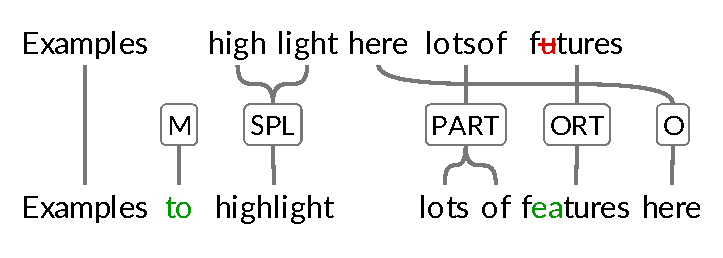
\includegraphics[height=2.0cm, trim={-0.5cm 0.55cm 0 0}, clip]{features7.pdf}
\caption{Example annotated sentence using ASK taxonomy. From left to right:
missing word, oversplitting, overcompounding, orthographic deviation and
word order.
\label{fig:normann}}
\end{figure}


For simplicity the labels range over an entire connected
component in the graph.
\footnote{Should this level of granularity prove too restrictive
it can be lifted to allow labelling individual edges or tokens.}

By putting the labels on components of edges
(rather than the alternative to put them on the source tokens) gives the advantage that any part of the interface can be used to annotate the norm deviations:
the user may click words in the source text and choose a norm deviation label from a menu. Or, they can click on the graph directly. Or in any of the other two panes,
since they are all connected via the links.
Further, insertions (due to missing words) do not correspond to any token in the source text so it would not work to only put labels on the source text.

The norm deviation annotation can be done after normalising the text, but annotators can go back and forth between the modes
if they want to improve the normalisation.

For ergonomics, when using the tool for several hours a day,
we also provide keyboard bindings for labelling and navigating between
the linked components.
% \mats{Det här passar kanske bättre i föregående sektion, Dan?}
We can improve the user experience by allowing the annotator to connect
and disconnect links directly in the ladder diagram.
% This should also be possible by using keyboard shortcuts in the editor.
% Frequent operations such as transposing words can also get dedicated keyboard bindings.

A preliminary error annotation could automatically be inferred.
For example, in a suffixing language like Swedish we can automatically
suggest revelant labels when noticing changes in common suffixes for tense
or definiteness.
Many deviation labels are easy to infer even without any linguistic
insight: missing or redundant words, deviant word order, overcompounding
and oversplitting.
This is something that we plan to explore further later on in the project.
% More herustics for automatic label suggestion can be done independently of the rest of the
% user interface, like a plugin, and more heuristics can be added as the
% project continues.

Note that we can use the same system for anonymizing the text by setting a
special anonymization label. An anonymised version of the corpus stripped
out of source tokens connected to such an anonymisation label may be released.\dan{move to discussion}

\section{Discussion}
\label{sec:discussion}

% Summarise overall workflow\ldots ?
% \elena{Merge together Disussion and Conclusions for now?}

Although only the normalisation component of \normAnn has been finsished so far, we have good reason to believe that transformation-based annotation of norm deviations, along with a coherent set of categories for norm deviations and a detailed guideline, will increase the efficiency and consistency by minimising subjectivity and increasing interannotator agreement. \dan{Because:}
First, the conceptually different tasks of deciding on a target hypotheses (with resulting normalisations) and annotating norm deviations are separated.
Also, since the source text and normalised text are displayed in separate panes, with the normalised text being incrementally updated, the annotator has access to all the relevant information for familiarising themselves with the specific interlanguage of the learner, and thus to make consistent decisions on target hypotheses.
In addition, the process could be made more efficient by inferring a preliminary error annotation from the editing operations. An additional advantage is that a parallel text is incrementally constructed based on the editing operations, thereby allowing for search in either or both of the source and normalised texts, and training of systems for automated annotation of norm deviations \cite{sproat2016rnn}.
We expect our approach to be useful also for other kinds of problems which involve parallel texts and manual annotation, such as text simplification, standardisation of short message texts, essay-grading by teachers and linguistic typology. % or peer-reviewers.

%We anticipate that our approach could also be useful for other problems which are based on parallel texts and systematic differences between them are vital for developing automated tools for the purpose, e.g. text simplification, standardizing short message texts, or essay-grading by teachers or peer-reviewers. % for personal or online (collaborative ?) feedback (teachers/peer reviewers suggesting better rewriting of a learner's text (e.g. Lo, Wang and Yeh (2008) and Yeh and Lo (2009) for their Online Annotator for EFL Writing say   “that online annotation functionalities for manipulating, rearranging, search, displaying and sharing annotations can be used to support EFL error correction and corrective feedback, especially the collaboration between teachers and students outside the classroom” (p. 883))...

%\section{Conclusion}
%\label{sec:conclusions}

%Your submission of a finalised contribution for inclusion in the LREC
%proceedings automatically assigns the above-mentioned copyright to ELRA.

\section{Acknowledgements}

This work has been supported by an infrastructure grant from Riksbankens Jubileumsfond (SweLL -- Research Infrastructure for Swedish as a Second Language, project IN16-0464:1). The ideas advanced here owe much to an earlier pilot developed by Felix Hultin \cite{correctAnnotator}, supervised by Robert Östling and Mats Wirén. We have received valuable comments and feedback on the tool from Markus Forsberg, Lars Borin and Beáta Megyesi.

\begin{comment}
\section{Providing References}

\subsection{Bibliographical References}
Bibliographical references should be listed in alphabetical order at the
end of the article. The title of the section, ``Bibliographical References'',
should be a level 1 heading. The first line of each bibliographical reference
should be justified to the left of the column, and the rest of the entry should
be indented by 0.35 cm.

The examples provided in Section \secref{main:ref} (some of which are fictitious
references) illustrate the basic format required for articles in conference
proceedings, books, journal articles, PhD theses, and chapters of books.

\subsection{Language Resource References}

Language resource references should be listed in alphabetical order at the end
of the article, in the \textbf{Language Resource References} section, placed after
the \textbf{Bibliographical References} section. The title of the ``Language Resource
References'' section, should be a level 1 heading. The first line of each
language resource reference should be justified to the left of the column, and
the rest of the entry should be indented by 0.35 cm. The example in Section
\secref{lr:ref} illustrates the basic format required for language resources.

In order to be able to cite a language resource, it must be added to
the \texttt{.bib} file first, as a \texttt{@LanguageResource} item type, which
contains the following fields:

\begin{itemize}
    \item{\texttt{author}: the builder of the resource}
    \item{\texttt{title}: the name of the resource}
    \item{\texttt{publisher}: the publisher of the resource (project,
          organisation etc)}
    \item{\texttt{year}: year of the resource release}
    \item{\texttt{series}: more general resource set this language resource
          belongs to}
    \item{\texttt{edition}: version of the resource}
    \item{\texttt{islrn}: the International Standard Language Resource Number
          (ISLRN) of the resource\footnote{The ISLRN number is available from
          \texttt{http://islrn.org}}}
\end{itemize}

If you want the full resource author name to appear in the citation, the
language resource author name should be protected by enclosing it between
\texttt{\{...\}}, as shown in the model \texttt{.bib} file.

\vspace{.3\baselineskip}

\section*{Appendix: How to Produce the \texttt{.pdf} Version}

In order to generate a PDF file out of the LaTeX file herein, when citing
language resources, the following steps need to be performed:

\begin{itemize}
    \item{Compile the \texttt{.tex} file once}
    \item{Invoke \texttt{bibtex} on the eponymous \texttt{.aux} file}
    \item{Invoke \texttt{bibtex} on the \texttt{languageresources.aux} file}
    \item{Compile the \texttt{.tex} file twice}
\end{itemize}
\end{comment}

% \nocite{*}
\section{Bibliographical References}
\label{main:ref}

\bibliographystyle{lrec}
\bibliography{xample}

% \section{Language Resource References}
% \label{lr:ref}
% \bibliographystylelanguageresource{lrec}
% \bibliographylanguageresource{xample}

\end{document}
